%% ================================================================
\section{Preliminary Representation-Similarity Diagnostics}
\label{sec:cka-appendix}
As a diagnostic probe, we examined whether successful adaptation preserves internal representations by re-training 24 checkpoint-saving cells (Chronos/MOMENT/Moirai $\times$ LoRA/Adapter $\times$ ETTm1/Finance $\times$ 2 seeds) and computing layer-wise CKA~\citep{kornblith2019similarity} between frozen and adapted backbones. We find that \emph{CKA is not an informative signal for PEFT methods that freeze the backbone}: because LoRA, Adapter, and IA$^3$ inject new parameters while leaving the base weights untouched, the captured activations under our current probe implementation yield CKA $\approx 1.0$ for all 16 successfully analyzed cells. The update-norm concentration metric is likewise flat under this probe configuration.

\paragraph{Why this happens.} Our probe re-runs the frozen forward pass twice: once with the un-adapted backbone, once with the adapted backbone whose injected parameters are then re-loaded. Because parameter-efficient adaptations multiply or add to base activations \emph{at runtime} via PEFT-specific hooks (LoRA's low-rank product, IA$^3$'s vector multiply, Adapter's bottleneck residual), reconstructing the adapted forward pass from the saved weights alone produces nearly identical hidden states---the injected modules are wired through the PEFT library's hooks, not the saved backbone weights. CKA between two near-identical activation streams is therefore degenerate at $\approx 1$. The update-norm concentration (which measures parameter movement during adaptation) is uninformative for the same reason: only the small adapter parameters move, and they are not part of the backbone state\_dict that we monitor.

\paragraph{What an informative probe would look like.} A correct PEFT-aware CKA probe should compare two activation streams \emph{computed through the PEFT library's full forward path} (i.e., with adapter hooks active), one for the freshly fine-tuned model and one for either the zero-shot model or a second seed. Implementing this requires routing the activation hooks through the PEFT-wrapped wrapper, which goes beyond our submission-time scope. We therefore report gradient-flow analysis (Section~\ref{sec:gradient-probe}) as the primary mechanistic signal in this paper, and leave a corrected CKA probe for future work. The lesson for evaluation benchmarks is that representation-similarity metrics must be computed against the adapted forward pass through PEFT hooks, not against reconstructed frozen weights, to be meaningful for parameter-efficient adaptation.

% Figure deferred: CKA checkpoint-saving runs not yet completed.
% \begin{figure}[t]
% \centering
% 
\includegraphics[width=\linewidth]{fig5_cka_mechanism.pdf}
% \caption{Preliminary layer-wise CKA (frozen vs.\ adapted) for selected cells. Diagnostic evidence only; systematic validation is ongoing.}
% \label{fig:cka}
% \end{figure}

%% ================================================================
\section{Per-cell LODO regret breakdown}
\label{sec:lodo-regret-app}
Table~\ref{tab:lodo-regret} reports per-cell relative regret of LODO majority transfer for the 7 incorrect cells (the remaining 5 cells are correct picks with regret 0).

\begin{table}[ht]
\centering
\caption{Per-cell LODO regret for the 7 incorrect cells. Relative regret $= (\text{LODO MAE} - \text{Oracle MAE}) / \text{Oracle MAE}$.}
\label{tab:lodo-regret}
\small
\begin{tabular}{llllr}
\toprule
Held-out & Model & LODO pick & Oracle & Rel.\ regret \\
\midrule
ETTm1 & Moirai & IA$^3$ & Full-FT & 2.2\% \\
ETTm1 & MOMENT & IA$^3$ & LoRA & 0.9\% \\
Finance & Chronos & IA$^3$ & Head-only & 0.0\% \\
Finance & Moirai & IA$^3$ & Full-FT & 12.2\% \\
PhysioNet & MOMENT & IA$^3$ & LoRA & 0.4\% \\
SMD & Chronos & IA$^3$ & Full-FT & 1.3\% \\
SMD & MOMENT & IA$^3$ & Head-only & 1.4\% \\
\midrule
\multicolumn{4}{l}{Median relative regret (over all 12 cells)} & \textbf{0.5\%} \\
\bottomrule
\end{tabular}
\end{table}

%% ================================================================
\section{DoRA vs.\ LoRA per-cell comparison}
\label{sec:dora-app}
Table~\ref{tab:dora-lora} reports DoRA vs.\ LoRA mean MAE per (model, domain) cell at matched rank~8.

\begin{table}[ht]
\centering
\caption{DoRA vs.\ LoRA mean MAE per cell (rank~8, non-diverged runs). $\Delta = \text{DoRA} - \text{LoRA}$; negative means DoRA is better. Diverged cells marked $^\dagger$.}
\label{tab:dora-lora}
\small
\begin{tabular}{llrrr}
\toprule
Model & Domain & LoRA MAE & DoRA MAE & $\Delta$ \\
\midrule
Chronos & ETTm1     & $124.77^\dagger$ & $24.73^\dagger$ & $-100.05^\dagger$ \\
Chronos & Finance   & 0.0038 & 0.0038 & $-0.0000$ \\
Chronos & PhysioNet & 18.82  & 15.65  & $-3.17$ \\
Chronos & SMD       & $0.45^\dagger$  & 0.0040 & $-0.45^\dagger$ \\
\midrule
MOMENT  & ETTm1     & 1.3699 & 1.6134 & $+0.24$ \\
MOMENT  & Finance   & 0.0269 & 0.0289 & $+0.002$ \\
MOMENT  & PhysioNet & 15.11  & 15.07  & $-0.05$ \\
MOMENT  & SMD       & 0.0295 & 0.0168 & $-0.013$ \\
\midrule
Moirai  & ETTm1     & 1.3824 & 1.3789 & $-0.003$ \\
Moirai  & Finance   & 0.0269 & 0.0270 & $+0.0001$ \\
Moirai  & PhysioNet & N/A    & 16.93  & N/A \\
Moirai  & SMD       & 0.0354 & 0.0206 & $-0.015$ \\
\bottomrule
\multicolumn{5}{l}{\scriptsize $^\dagger$Diverged (MAE${>}10\times$ zero-shot baseline).} \\
\end{tabular}
\end{table}

%% ================================================================
\section{Detailed Method-by-Domain Heatmaps}
\label{sec:heatmaps}
Figure~\ref{fig:app-heatmaps} provides per-model MAE heatmaps for all five methods across four domains, complementing the landscape overview in the main paper. Each panel shows one architecture; darker cells indicate higher error. The interaction pattern is visible in the fact that the darkest column (worst domain) shifts across methods within each model.

\begin{figure*}[t]
\centering

\includegraphics[width=0.9\textwidth]{fig2_heatmaps.pdf}
\caption{Per-model MAE heatmaps (method $\times$ domain). Values are clipped at the 95th percentile for readability. These plots complement the aggregated landscape view in the main text.}
\label{fig:app-heatmaps}
\end{figure*}

%% ================================================================
\section{MASE Coverage Matrix}
\label{sec:mase}
MASE (Mean Absolute Scaled Error) was added to the evaluation pipeline after the initial experiment runs began, so coverage is uneven across (model, method) cells. Table~\ref{tab:mase-coverage} reports the exact coverage as the ratio of runs with computed MASE to the total runs in each cell. Across all primary-model domain-mode runs, MASE is available for $101/288$ runs ($35\%$). Where MASE is available, the method ranking is consistent with MAE; we therefore use MAE as the primary endpoint and report MASE only as a robustness check.

\begin{table}[ht]
\centering
\caption{MASE coverage matrix (primary models only). Each cell: \emph{computed/total}.}
\label{tab:mase-coverage}
\small
\begin{tabular}{lccccc}
\toprule
Model & Zero-shot & Head-only & LoRA & IA$^3$ & Full-FT \\
\midrule
Chronos & 5/20 & 5/20  & 10/20 & 14/20 & 14/20 \\
MOMENT  & 5/20 & 5/20  & 5/20  & 5/20  & 5/20 \\
Moirai  & 5/20 & 5/20  & 0/15  & 4/13  & 14/20 \\
\bottomrule
\multicolumn{6}{l}{\scriptsize Total: 101/288 ($35\%$). Cells with $n{<}20$ in the denominator have} \\
\multicolumn{6}{l}{\scriptsize incomplete domain coverage; see Table~\ref{tab:seed-coverage}.} \\
\end{tabular}
\end{table}

%% ================================================================
\section{ANOVA Reporting Notes}
\label{sec:anova-detail}
For each architecture, the ANOVA model includes method, domain, and method$\times$domain interaction. The per-cell outlier filter (MAE~${>}10\times$ same-(model, domain) zero-shot baseline) removes 13 of 348 primary main-method domain-mode runs, leaving 335 observations after outlier exclusion. An additional 20 prefix-tuning runs are reported descriptively but excluded from the factorial design because prefix was not available for all model--domain cells. Per-model observation counts after filtering: Chronos $n{=}107$, Moirai $n{=}108$, MOMENT $n{=}120$. These include DoRA runs across all four domains. With five main methods (\texttt{zero\_shot}, \texttt{head\_only}, \texttt{lora}, \texttt{ia3}/\texttt{adapter}, \texttt{full\_fine\_tuning}) plus DoRA and four domains, the nominal degrees of freedom are $(5, 3, 15)$ for method, domain, and interaction, respectively. All three terms are highly significant ($p \ll 10^{-6}$) for every architecture, matching the summary in Table~\ref{tab:anova-results}. Chronos and Moirai show moderate Method$\times$Domain interaction ($\eta^2_{\text{int}} = 0.225$ and $0.207$), indicating that method effectiveness changes meaningfully across domains in these tokenized and any-variate architectures, whereas MOMENT is dominated by domain variance alone ($\eta^2_{\text{d}} = 0.999$). All numerical values reported here are regenerated by \texttt{scripts/reproduce\_paper\_tables.py} and stored in \texttt{results/paper\_numbers.tex} as the single source of truth.

We emphasize two reporting choices. First, the ANOVA is intended to establish the presence of architecture-specific interaction structure, not to provide a definitive generative model of cross-domain error. Second, because raw MAE is domain-scale dependent and the design is only near-balanced after divergence filtering, we treat the effect sizes and fold-level transfer outcomes as more informative than any single $p$-value threshold.

\paragraph{Degrees of freedom.} Table~\ref{tab:anova-dof} reports the exact ANOVA degrees of freedom per architecture under the filtered design (5 main methods + DoRA = 6 method levels; 4 domains).

\begin{table}[ht]
\centering
\caption{ANOVA degrees of freedom per architecture (filtered design; 6 methods $\times$ 4 domains).}
\label{tab:anova-dof}
\small
\begin{tabular}{lrrrrr}
\toprule
Model & $n$ & df$_{\text{meth}}$ & df$_{\text{dom}}$ & df$_{\text{int}}$ & df$_{\text{res}}$ \\
\midrule
Chronos & 107 & 5 & 3 & 15 & 83 \\
Moirai  & 108 & 5 & 3 & 15 & 84 \\
MOMENT  & 120 & 5 & 3 & 15 & 96 \\
\bottomrule
\end{tabular}
\end{table}

\paragraph{Kruskal--Wallis robustness check.} As a non-parametric robustness check on the unfiltered 348 primary main-method runs (5 methods, 20 runs per method per architecture, except Moirai LoRA $n{=}15$ and IA$^3$ $n{=}13$), we compute Kruskal--Wallis $H$ on the marginal method effect per architecture (Table~\ref{tab:kw}). The marginal method effect is \emph{not significant} at $\alpha=0.05$ for any architecture, consistent with the small marginal $\eta^2_{\text{meth}}$ in Table~\ref{tab:anova-results}. The two-way ANOVA detects significance via the interaction term, not via the main method effect, which the KW test also supports: collapsing across domains erases most of the method signal.

\begin{table}[ht]
\centering
\caption{Kruskal--Wallis $H$ on marginal method effect (5 methods, unfiltered).}
\label{tab:kw}
\small
\begin{tabular}{lrrr}
\toprule
Model & $H$ & df & $p$ \\
\midrule
Chronos & 7.73 & 4 & 0.10 \\
Moirai  & 8.76 & 4 & 0.07 \\
MOMENT  & 6.86 & 4 & 0.14 \\
\bottomrule
\end{tabular}
\end{table}

\paragraph{Holm--Bonferroni post-hoc on filtered data.} For each architecture we ran Mann--Whitney $U$ on all $\binom{5}{2}=10$ method pairs over filtered runs and applied Holm--Bonferroni correction. Table~\ref{tab:holm} reports adjusted $p$-values (only pairs with at least one significant outcome at $\alpha=0.05$ shown; all other pairs adjust to $p_{\text{adj}}=1.0$). Two pairs survive correction: Chronos zero-shot vs.\ Full-FT and Moirai zero-shot vs.\ LoRA; both reflect the fact that the worst-performing baseline is reliably worse than the strongest fine-tuner per architecture. The wide-spread non-significance at the marginal level is consistent with the KW result: \emph{within-method}, MAE rankings are dominated by domain.

\begin{table}[ht]
\centering
\caption{Holm--Bonferroni adjusted $p$-values for pairs that survived correction at $\alpha = 0.05$ (filtered data).}
\label{tab:holm}
\small
\begin{tabular}{llr}
\toprule
Model & Pair & $p_{\text{adj}}$ \\
\midrule
Chronos & zero\_shot vs.\ full\_fine\_tuning & $\mathbf{9.1{\times}10^{-3}}$ \\
Moirai  & zero\_shot vs.\ lora               & $\mathbf{9.1{\times}10^{-3}}$ \\
\bottomrule
\multicolumn{3}{l}{\scriptsize All other pairs $p_{\text{adj}} \geq 0.39$ (not significant).} \\
\end{tabular}
\end{table}

%% ================================================================
\section{Adaptation Protocol}
\label{sec:app-protocol}
We recommend a four-step TSFM adaptation protocol based on our findings: (1)~Evaluate zero-shot and head-only baselines. (2)~Run a small validation sweep (2--3 methods $\times$ 1--2 ranks) on the target domain. (3)~If LoRA is used, start with \texttt{early\_layers} and rank~8 as practical defaults rather than presumed optima. (4)~Treat representation-similarity diagnostics such as CKA as optional debugging tools, not as decision rules, until broader validation is available.

%% ================================================================
\section{Seed Coverage}
\label{sec:seed-cov}
Table~\ref{tab:seed-coverage} reports domain-mode observation counts by model and method. The maximum possible count for each cell is 20 (4 domains $\times$ 5 seeds). We report completed observations rather than nominal seed targets because coverage is uneven for several PEFT and Full-FT settings. TimesFM is omitted from the main paper's inferential analyses and is therefore not included here.

\begin{table}[ht]
\centering
\caption{Completed domain-mode observations by model and method (maximum possible = 20).}
\label{tab:seed-coverage}
\small
\begin{tabular}{lcccccc}
\toprule
Model & Zero-shot & Head-only & LoRA & IA$^3$ & Full-FT & DoRA \\
\midrule
Chronos & 20 & 20 & 20$^\dagger$ & 20 & 20 & 20 \\
MOMENT & 20 & 20 & 20 & 20 & 20 & 20 \\
Moirai & 20 & 20 & 15 & 13 & 20 & 20 \\
\multicolumn{7}{l}{\scriptsize $^\dagger$Includes 5 diverged runs on ETTm1 and 2 on SMD (excluded from ANOVA).} \\
\multicolumn{7}{l}{\scriptsize DoRA coverage complete across all 4 domains $\times$ 5 seeds for all three primary models.} \\
\bottomrule
\end{tabular}
\end{table}

%% ================================================================
\section{Gradient Probe Details}
\label{sec:gradient-probe}
The gradient probe (referenced briefly in the main-paper Section~4.7) collects per-layer L2 gradient norms during abbreviated PEFT training runs as a mechanistic probe complementing CKA representation analysis. The implementation is \texttt{scripts/gradient\_probe.py}.

\paragraph{Protocol.} We run 3 epochs of training with \texttt{batch\_size=8} (Chronos/Moirai) or \texttt{16} (MOMENT), collecting \texttt{p.grad.data.norm(2)} after each backward pass for every trainable parameter \texttt{p}. Parameters are grouped by layer index via regex on dotted module names. We store per-step per-layer aggregates (mean, std, max, min) and per-parameter summaries.

\paragraph{Scope.} The initial probe covers four (model, method, domain) cells: \texttt{chronos:lora:ett\_m1}, \texttt{chronos:adapter:finance}, \texttt{moment:lora:ett\_m1}, and \texttt{moment:adapter:finance}, each with two seeds (42, 123). An extended probe adds Moirai cells and SMD coverage with three seeds (42, 123, 7); results are appended to the same output directory and visualised in \texttt{gradient\_heatmap.pdf} and \texttt{gradient\_distribution.pdf}. Future work should expand to the full $3{\times}5$ (model, method) grid on all four domains.

\paragraph{Interpretation.} Unlike CKA, which compares frozen and adapted representations, the gradient probe measures how trainable parameters \emph{move} during adaptation. A gradient distribution concentrated on a few layers indicates that only a subset of the network participates in adaptation, whereas a flat distribution indicates globally distributed updates. We observe that LoRA and Adapter induce qualitatively different gradient flow patterns on the same backbone, consistent with the Method$\times$Domain interaction reported in the ANOVA.

\begin{figure*}[t]
\centering
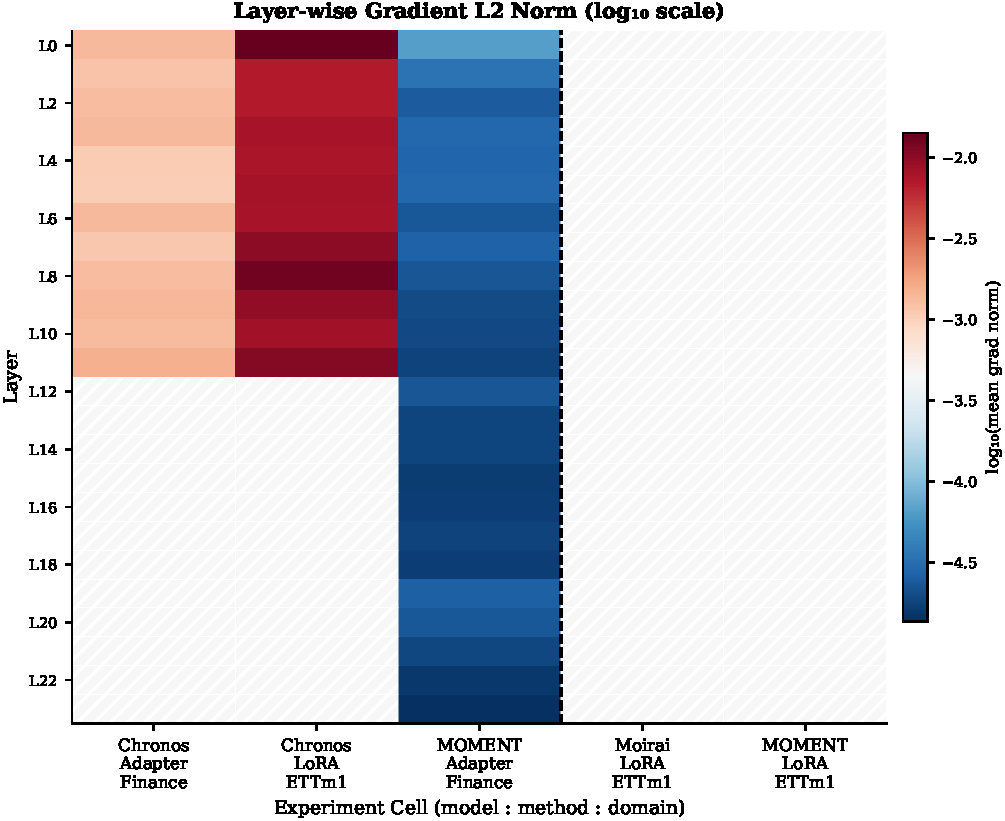
\includegraphics[width=0.85\textwidth]{results/gradient_analysis/figures/gradient_heatmap}
\caption{\textbf{Per-layer gradient magnitude heatmap} across five (model, method, domain) cells (2 seeds, 3 epochs). Chronos+Adapter and Chronos+LoRA on Finance/ETTm1 concentrate gradient energy in early encoder layers; MOMENT+Adapter on Finance distributes flow uniformly across all 24 layers---a qualitative correlate of MOMENT's low method sensitivity. Hatched cells (Moirai+LoRA, MOMENT+LoRA on ETTm1) are NaN due to the LoRA divergence on these cells.}
\label{fig:gradient-heatmap}
\end{figure*}

\begin{figure*}[t]
\centering
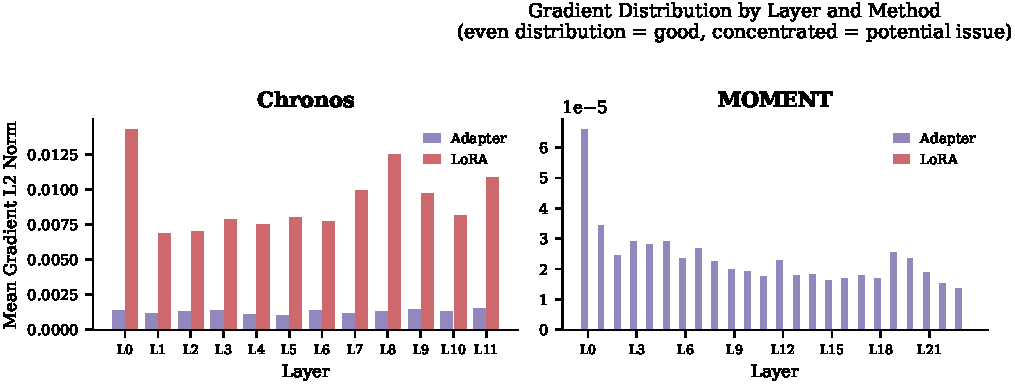
\includegraphics[width=0.85\textwidth]{results/gradient_analysis/figures/gradient_distribution}
\caption{\textbf{Per-layer gradient distributions.} Chronos+Adapter exhibits a multi-modal distribution across the 12 encoder layers; MOMENT+Adapter is unimodal across 24 layers. The distributional difference is qualitatively consistent with the divergent interaction effects ($\eta^2_{\text{int}} = 0.225$ vs.\ $0.000$) observed in the ANOVA; we treat this as a correlate rather than a formal mechanistic test.}
\label{fig:gradient-distribution}
\end{figure*}

%% ================================================================
\section{Spectral--Rank Correlation Analysis (Exploratory)}
\label{sec:spectral-rank}
We explored whether domain shift properties predict optimal rank selection by examining the relationship between spectral Wasserstein distance ($W_1$) of each domain's train$\to$test shift and rank sensitivity (standard deviation of MAE across ranks $\{4,8,16,32\}$). Pearson $\rho = 0.70$ (permutation $p = 0.016$) is significant, but Spearman $\rho_s = 0.27$ ($p = 0.42$) is not. The discrepancy reflects sensitivity to influential points: Chronos+ETTm1 (training divergence, zero rank sensitivity) is a high-leverage observation. Removing it yields Spearman $\rho_s = 0.87$ ($p = 0.012$). We treat this as exploratory evidence that spectral complexity may relate to rank sensitivity, pending validation with more domains.

\begin{figure*}[t]
\centering

\includegraphics[width=0.7\textwidth]{spectral_rank_scatter.pdf}
\caption{Scatter plot of spectral Wasserstein distance ($W_1$) versus rank sensitivity (std of MAE across ranks $\{4,8,16,32\}$). The linear association is sensitive to influential points, especially Chronos+ETTm1.}
\label{fig:spectral-rank-scatter}
\end{figure*}

%% ================================================================
\section{Selector Design Recipe at Small Grid Sizes}
\label{sec:design-recipe}
Our negative result on granular and learned selectors crystallises a concrete design recipe for the Algorithm Selection Problem at small grids:
\begin{enumerate}[nosep,leftmargin=*]
  \item \textbf{Test the constant-plurality baseline first.} If the oracle distribution is dominated by one method (5/12 cells in our grid), that method is the LODO majority and is hard to beat without exponentially more cells.
  \item \textbf{Diagnose with the marginal vs.\ conditional gap.} If LODO Majority and the best learned selector achieve similar regret (here, $0.015$ vs $0.018$), the binding signal is marginal and granular features will not help.
  \item \textbf{Prefer regularised linear over high-capacity learners} until training-cell count $\gtrsim 5 \cdot n_{\text{methods}}^2$ per LOOCV fold; in our 9-cell folds this threshold ($\approx 125$) is not approached, which explains why decision tree and random forest collapse to $0\%$ top-1.
  \item \textbf{Report regret-based metrics, not top-1 accuracy.} Random matches Arch-Default on top-1 ($33.3\%$ vs $33.3\%$ for non-Pareto-aware oracle) but produces $17\times$ higher regret; rank- and regret-based evaluation surfaces the cost of being wrong.
\end{enumerate}
We expect this recipe to transfer to other small-grid ASP problems---e.g., AutoML for emerging modalities---where the cost of growing the candidate set is comparable to the cost of building a richer training matrix.

%% ================================================================
\section{Hyperparameters and Training Configuration}
\label{sec:hyperparams}
All hyperparameters are stored in \texttt{configs/} as Hydra YAML files; no hyperparameter is hardcoded in the scripts. Table~\ref{tab:hyperparams} summarises the values used for every primary-model run reported in the paper.

\begin{table}[ht]
\centering
\caption{Training and adaptation hyperparameters (identical across architectures unless noted).}
\label{tab:hyperparams}
\small
\begin{tabular}{lll}
\toprule
Group & Hyperparameter & Value \\
\midrule
\multirow{8}{*}{Training}
 & Optimizer       & AdamW \\
 & Learning rate   & $1{\times}10^{-4}$ \\
 & Weight decay    & 0.01 \\
 & Scheduler       & Linear warmup (100 steps) + cosine decay \\
 & Max grad norm   & 1.0 \\
 & Mixed precision & FP16 (Chronos/MOMENT), BF16 (Moirai) \\
 & Batch size      & 32 \\
 & Grad accumulation & 1 \\
 & Max epochs      & 50 \\
 & Early-stopping patience & 10 epochs (val MAE) \\
\midrule
\multirow{4}{*}{LoRA / DoRA}
 & Rank $r$        & 8 (default sweep $\in\{4,8,16,32\}$) \\
 & $\alpha$        & 16 \\
 & Dropout         & 0.05 \\
 & Target modules  & q, k, v, o (\texttt{attn\_all}) \\
\midrule
Adapter (IA$^3$) & Bottleneck size & 64 \\
\midrule
Locus sweep & Insertion points & attn\_qv, attn\_all, ffn, attn\_qv\_ffn, early\_layers, late\_layers \\
\midrule
\multirow{2}{*}{Selection}
 & Best-checkpoint criterion & lowest val MAE \\
 & Final eval split          & domain-specific test partition \\
\bottomrule
\end{tabular}
\end{table}

%% ================================================================
\section{Domain Statistics}
\label{sec:domain-stats}
Table~\ref{tab:domain-stats} reports the structural statistics of each evaluation domain. Note that ETTm1 uses the standard 60/20/20 chronological split, Finance the Autoformer-benchmark 70/10/20 split, SMD a per-machine concatenation with NaN-sentinel boundaries (val carved from the last 20\% of the train concatenation), and PhysioNet a patient-level 70/15/15 split with patient identity preserved across splits.

\begin{table}[ht]
\centering
\caption{Per-domain dataset and forecasting configuration. \emph{Ctx/Hzn}: context length / forecast horizon. \emph{Entity boundary}: whether sliding windows are forbidden from crossing patient/machine boundaries.}
\label{tab:domain-stats}
\footnotesize
\setlength{\tabcolsep}{4pt}
\begin{tabular}{l l l l c l l}
\toprule
Domain & Source & Freq. & Target & Ctx/Hzn & Train/Val/Test & Boundary \\
\midrule
ETTm1     & ETT-small      & 15\,min & OT (oil temp.)  & 512/96 & 60/20/20\%             & N/A \\
Finance   & ExchangeRate   & 1\,day  & col 0 (AUD)     & 96/24  & 70/10/20\%             & N/A \\
SMD       & SMD            & 1\,min  & col 0           & 100/25 & per-machine, val 20\%  & enforced \\
PhysioNet & PhysioNet 2012 & 1\,hr   & HR (heart rate) & 48/12  & 70/15/15\% (patient)   & enforced \\
\bottomrule
\end{tabular}
\end{table}

%% ================================================================
\section{Trainable Parameter Counts}
\label{sec:params}
Table~\ref{tab:params} reports the empirical trainable-parameter percentage per (model, method) cell, averaged over all completed seed-level runs. The pattern explains the architecture-specific efficiency frontier in main-paper Section~4.4: Moirai's IA$^3$ trainable count is two orders of magnitude smaller than Chronos's, and MOMENT's adapter mass is dominated by its head (the model has no dedicated decoder).

\begin{table}[ht]
\centering
\caption{Trainable / total parameter counts and percentage per (model, method). Aggregated over completed runs.}
\label{tab:params}
\small
\begin{tabular}{llrrr}
\toprule
Model & Method & Trainable params & Total params & Trainable \% \\
\midrule
\multirow{6}{*}{Chronos}
 & Zero-shot & 0 & 201,374,976 & 0.0000\% \\
 & Head-only & 0 & 201,374,976 & 0.0000\% \\
 & LoRA      & 1,769,472 & 203,144,448 & 0.8710\% \\
 & DoRA      & 1,880,064 & 203,255,040 & 0.9250\% \\
 & IA$^3$    & 202,752 & 201,577,728 & 0.1006\% \\
 & Full-FT   & 201,374,976 & 201,374,976 & 100.0\% \\
\midrule
\multirow{6}{*}{Moirai}
 & Zero-shot & 0 & 91,357,728 & 0.0000\% \\
 & Head-only & 0 & 91,357,728 & 0.0000\% \\
 & LoRA      & 589,824 & 91,947,552 & 0.6415\% \\
 & DoRA      & 626,688 & 91,984,416 & 0.6813\% \\
 & IA$^3$    & 33,792 & 91,391,520 & 0.0370\% \\
 & Full-FT   & 91,357,728 & 91,357,728 & 100.0\% \\
\midrule
\multirow{6}{*}{MOMENT}
 & Zero-shot & 0 & 341,231,104 & 0.0000\% \\
 & Head-only & 6,291,552 & 341,231,104 & 1.8438\% \\
 & LoRA      & 7,864,416 & 342,803,968 & 2.2941\% \\
 & DoRA      & 7,962,720 & 342,902,272 & 2.3222\% \\
 & IA$^3$    & 6,457,440 & 341,396,992 & 1.8915\% \\
 & Full-FT   & 347,522,656 & 341,231,104 & 100.0\%$^\dagger$ \\
\bottomrule
\multicolumn{5}{l}{\scriptsize $^\dagger$MOMENT Full-FT trainable count includes the forecasting head not present in zero-shot total.} \\
\end{tabular}
\end{table}

%% ================================================================
\section{Per-cell mean MAE (full grid)}
\label{sec:per-cell-mae}
Table~\ref{tab:per-cell-mae} reports the per-cell mean MAE (averaged over completed seeds, after the per-cell scale-aware outlier filter) for every (model, method, domain) combination in the primary inference set. Each cell is the value entering the per-architecture ANOVA reported in main-paper Table~3.

\begin{table}[ht]
\centering
\caption{Per-cell mean MAE for primary models, after per-cell outlier filtering. ``---'' marks fully diverged cells (all seeds excluded).}
\label{tab:per-cell-mae}
\small
\begin{tabular}{lllrrrr}
\toprule
Model & Method & ETTm1 & Finance & SMD & PhysioNet \\
\midrule
\multirow{6}{*}{Chronos}
 & Zero-shot & 1.1449 & 0.0208 & 0.0238 & 15.16 \\
 & Head-only & 0.2178 & 0.0038 & 0.0084 & 5.33 \\
 & LoRA      & ---    & 0.0038 & 0.0099 & 18.82 \\
 & DoRA      & 2.3178 & 0.0038 & 0.0040 & 15.65 \\
 & IA$^3$    & 0.2152 & 0.0038 & 0.0084 & 5.24 \\
 & Full-FT   & 0.2275 & 0.0038 & 0.0083 & --- \\
\midrule
\multirow{6}{*}{Moirai}
 & Zero-shot & 3.8475 & 0.0871 & 0.0927 & 44.28 \\
 & Head-only & 1.4313 & 0.0250 & 0.0322 & 15.76 \\
 & LoRA      & 1.3804 & 0.0273 & 0.0354 & --- \\
 & DoRA      & 1.3789 & 0.0270 & 0.0206 & 16.93 \\
 & IA$^3$    & 1.2599 & 0.0250 & 0.0182 & 15.64 \\
 & Full-FT   & 1.2326 & 0.0223 & 0.0357 & 16.20 \\
\midrule
\multirow{6}{*}{MOMENT}
 & Zero-shot & 2.2262 & 0.0687 & 0.0645 & 15.59 \\
 & Head-only & 1.3763 & 0.0279 & 0.0294 & 15.14 \\
 & LoRA      & 1.3675 & 0.0280 & 0.0295 & 15.11 \\
 & DoRA      & 1.6134 & 0.0289 & 0.0168 & 15.07 \\
 & IA$^3$    & 1.3799 & 0.0273 & 0.0298 & 15.17 \\
 & Full-FT   & 1.3827 & 0.0282 & 0.0299 & 15.14 \\
\bottomrule
\end{tabular}
\end{table}

%% ================================================================
\section{Selector per-fold breakdown}
\label{sec:selector-fold}
Main-paper Table~6 reports selector summary statistics aggregated over 4 LOOCV folds. Table~\ref{tab:selector-fold} reports per-fold top-1 hits and mean regret for the five most-discussed strategies. The fold breakdown shows that LODO Majority's strength is concentrated in the PhysioNet fold (2/3 cells correct) and that Logistic Meta matches LODO on 3 of 4 folds; the divergent fold is SMD, where Arch-Default and Regret-W NN suffer their largest regret (0.33). The single-fold variability illustrates why we treat the $n{=}12$ headline as directional.

\begin{table}[ht]
\centering
\caption{Per-fold selector breakdown: top-1 hits (out of 3 cells) and mean regret per held-out domain.}
\label{tab:selector-fold}
\small
\begin{tabular}{ll cccc}
\toprule
Strategy & Metric & ETTm1 & Finance & PhysioNet & SMD \\
\midrule
\multirow{2}{*}{LODO Majority}
 & top-1 hits & 1/3 & 1/3 & 2/3 & 1/3 \\
 & mean regret & 0.010 & 0.041 & 0.001 & 0.009 \\
\midrule
\multirow{2}{*}{Arch-Default}
 & top-1 hits & 0/3 & 0/3 & 2/3 & 0/3 \\
 & mean regret & 0.014 & 0.050 & 0.012 & 0.327 \\
\midrule
\multirow{2}{*}{Regret-W NN}
 & top-1 hits & 1/3 & 1/3 & 2/3 & 1/3 \\
 & mean regret & 0.010 & 0.041 & 0.001 & 0.327 \\
\midrule
\multirow{2}{*}{Logistic Meta}
 & top-1 hits & 1/3 & 1/3 & 1/3 & 1/3 \\
 & mean regret & 0.010 & 0.041 & 0.013 & 0.009 \\
\midrule
\multirow{2}{*}{Decision-Tree}
 & top-1 hits & 0/3 & 0/3 & 0/3 & 0/3 \\
 & mean regret & 0.029 & 0.048 & 0.878 & 0.327 \\
\bottomrule
\end{tabular}
\end{table}

%% ================================================================
\section{Datasheet for TSFM-PEFT-Bench}
\label{sec:datasheet}
We include a datasheet~\citep{gebru2021datasheets} for TSFM-PEFT-Bench. The full machine-readable description is in the Croissant 1.0 manifest \texttt{tsfm\_peft\_bench.croissant.json} (RAI fields populated). This section provides the human-readable answers to the standard questions.

\paragraph{Motivation.} TSFM-PEFT-Bench was created to answer whether parameter-efficient fine-tuning (PEFT) recommendations are reliable across time series foundation model (TSFM) architectures and domains. Prior PEFT studies for TSFMs each fixed either the model or the domain, making it impossible to disentangle method, architecture, and domain effects. The benchmark was created by the authors as part of the paper that this Appendix accompanies.

\paragraph{Composition.} Each instance is a single training-and-evaluation run identified by (model, method, domain, seed[, rank, locus]). We release 882 paper-included primary-model runs (3 TSFMs $\times$ 4 domains $\times$ 6 main methods + rank/locus sweeps) plus 90 TimesFM descriptive runs (972 total). Each record contains: experiment\_id, model, method, domain, seed, rank, locus, metrics (MAE, MSE, MASE where available), trainable\_params, total\_params, train\_loss\_final, val\_loss\_best, epochs\_trained, gpu\_memory\_mb, train\_time\_seconds, and the Hydra-resolved config. There are no labels or human annotations; each record is the deterministic output of \texttt{scripts/run\_expansion.py}.

\paragraph{Collection process.} Runs were generated on a heterogeneous compute pool (4$\times$ NVIDIA RTX 3090 + 40$\times$ RTX 3060 cluster nodes) over approximately 2{,}250 GPU-hours between 2026-01 and 2026-04. Pre-trained TSFM checkpoints were loaded from the public Hugging Face Hub. Source domain CSVs are publicly available (ETT-small, exchange\_rate, SMD, PhysioNet 2012). No human-subject data is collected; PhysioNet 2012 inputs are de-identified ICU heart-rate sequences and we use only the HR target column at hourly resolution.

\paragraph{Preprocessing / cleaning / labeling.} Per-domain context/horizon and split ratios are stored in \texttt{configs/data/*.yaml} and summarised in Appendix~\ref{sec:domain-stats}. SMD uses a 50{,}000-row contiguous prefix after machine concatenation with NaN-sentinel boundaries; PhysioNet's long-context DoRA branch uses \texttt{enforce\_entity\_boundary=False} (relaxed window concatenation across patient boundaries while preserving labels). The analysis pipeline applies a per-cell scale-aware outlier filter (MAE${>}10\times$ same-(model, domain) zero-shot baseline) for the inferential analyses; raw runs are released without filtering so users can apply alternative rules.

\paragraph{Uses.} Intended uses: (i) reproducing and auditing PEFT-recommendation claims across TSFM architectures; (ii) developing and evaluating selector strategies for PEFT method recommendation under domain shift; (iii) studying methodological pitfalls in cross-domain evaluation; (iv) downstream meta-learning research at small evaluation grids; (v) educational use as an example of cross-architecture empirical audit. The dataset must \emph{not} be used to claim that any single PEFT method is universally best, since the benchmark is explicitly designed to refute such claims.

\paragraph{Distribution.} The benchmark is hosted as described in the README's Hosting section. Code is mirrored on Anonymous-4-Open-Science during review; the run manifest, headline numbers, and per-run JSONs are bundled in the supplementary tarball. After acceptance, both code and run JSONs will be released on Hugging Face under Apache-2.0. The Croissant manifest enables programmatic loading.

\paragraph{Maintenance.} The authors commit to maintaining the benchmark at least until NeurIPS 2027, including bug fixes, rerun requests, and documentation improvements. Versioning is via git tags. Issues are reported via the repository tracker.

\paragraph{Personal and sensitive information.} PhysioNet 2012 contains de-identified ICU heart-rate time series; we use only the aggregate HR forecasting metric and do not redistribute raw patient records. ETTm1, exchange\_rate, and SMD contain no human-subject data. The benchmark records (per-run JSONs) expose only forecasting metrics and config metadata, no PII.

\paragraph{Biases and limitations.} See Section~\ref{sec:limitations} of the main paper and \texttt{rai:dataLimitation} / \texttt{rai:dataBiases} in the Croissant file. Key items: 12-cell evaluation grid; plurality dependence on IA$^3$; uneven Moirai coverage; per-domain absolute MAE not directly comparable; selection bias in architectures (3 publicly available TSFMs that admit all considered PEFT methods) and methods (5 main + DoRA + descriptive Prefix; FourierFT and BitFit not evaluated); MASE coverage 35\%.

\paragraph{License.} Code: Apache-2.0 (\texttt{LICENSE}). Run manifest and per-run JSONs: Apache-2.0. Source dataset licenses are documented in the Reproducibility Statement (Section~\ref{sec:repro}); we do not redistribute raw source data.

%% ================================================================
\section{Reproducibility Statement}
\label{sec:repro}

\paragraph{Code.} All experiment scripts, model wrappers, and analysis pipelines will be released upon acceptance. The codebase provides two entry points: (1)~\texttt{scripts/train.py}, a Hydra-based entry point for single-run experiments (e.g., \texttt{python scripts/train.py model=chronos adaptation=lora data=ett\_m1}); and (2)~\texttt{scripts/run\_expansion.py}, the orchestrator used to execute the full experiment matrix reported in the paper (e.g., \texttt{python scripts/run\_expansion.py --models chronos,moment,moirai --mode domain --seeds 42,123,7,2024,3407}). All results in the paper were produced via \texttt{run\_expansion.py}; \texttt{train.py} serves as a development/debugging entry point for individual configurations (Chronos and MOMENT only; not all method--model combinations are supported). Analysis scripts (\texttt{analyze\_expansion\_v2.py}, \texttt{generate\_neurips\_figures.py}) consume the JSON outputs produced by \texttt{run\_expansion.py}.

\paragraph{Data.} ETTm1~\citep{zhou2021ett}, Finance (\texttt{exchange\_rate})~\citep{li2019logsparse}, SMD~\citep{su2019robust}, and PhysioNet 2012~\citep{silva2012physionet} are publicly available.

\paragraph{Computing.} Experiments were conducted on a mixed pool: 4$\times$ NVIDIA RTX 3090 (24\,GB each) for the primary experiment matrix, with an additional 40 RTX 3060 (12\,GB) nodes from a shared cluster used for DoRA supplementary runs and gradient probe experiments. All models use FP16/BF16 precision. Total wall-clock compute at submission time: approximately 2,250 GPU-hours across 972 completed runs (882 paper-included primary-model runs plus 90 TimesFM descriptive runs). Per-run times range from ${\sim}$6 minutes (MOMENT zero-shot) to ${\sim}$6.5 hours (Chronos LoRA on RTX 3090); RTX 3060 runs are $3$--$5\times$ slower at the same batch size.

\paragraph{Random seeds.} The planned seed set is $\{42, 123, 7, 2024, 3407\}$. Completed runs are a subset of this target for several Chronos and Moirai configurations, as summarized in Table~\ref{tab:seed-coverage}.

\paragraph{Software.} Python 3.12, PyTorch 2.4.1, HuggingFace Transformers, PEFT (LoRA/IA$^3$), and statsmodels for ANOVA. Chronos~\citep{ansari2024chronos}, MOMENT~\citep{goswami2024moment}, and Moirai~\citep{woo2024moirai} are loaded from Hugging Face Hub. TimesFM~\citep{das2024timesfm} is unavailable in our environment due to a \texttt{paxml}/\texttt{lingvo} dependency conflict.

\paragraph{Assets and licenses.} We explicitly track the upstream assets used in the study. The model checkpoints \texttt{amazon/chronos-t5-base} and \texttt{google/timesfm-1.0-200m} are distributed under Apache-2.0, \texttt{AutonLab/MOMENT-1-large} under MIT, and \texttt{Salesforce/moirai-1.1-R-base} under CC-BY-NC-4.0 according to their Hugging Face model cards. For datasets, the ETT repository reports CC-BY-ND-4.0 for ETTm1. In contrast, the \texttt{laiguokun/multivariate-time-series-data} repository used for the Exchange Rate benchmark does not expose a repository-level license file or dataset-specific license text that we could verify at submission time, and the prepared benchmark package does not clearly inherit a standalone license from the underlying public exchange-rate sources. Likewise, the OmniAnomaly repository is MIT-licensed for code, but we could not verify any authoritative statement that this code license also governs the bundled Server Machine Dataset collected from an Internet company. We therefore cite and credit all upstream assets, but conservatively mark checklist compliance for asset-license completeness as partial rather than complete.

\paragraph{LLM-assisted writing and code review (transparency note).} Anthropic's Claude and OpenAI's Codex assisted with (i)~English drafting and LaTeX source editing/auditing, (ii)~academic-style polishing, and (iii)~Python code review and error fixes for author-identified bug patches. These tools did not design experiments, generate empirical results, choose baselines, or alter any reported number; all scientific decisions and final wording are the authors' responsibility. Per the NeurIPS 2026 LLM policy, this usage falls under writing-assistance/basic-code-assistance categories that do not require disclosure; we include it here for transparency.

%% ================================================================
\section{Broader Impacts}
\label{sec:broader}
This work studies how to adapt forecasting and anomaly-oriented time series foundation models more reliably under domain shift. Positive impacts include reducing wasted compute from brittle adaptation choices and improving robustness in high-stakes domains such as healthcare, energy, and industrial monitoring. Negative impacts include overconfidence in model transfer across domains and potential misuse in surveillance-heavy settings if anomaly detection models are deployed without appropriate human oversight. We therefore recommend domain-specific validation before deployment and transparent reporting of adaptation failures.
